\documentclass[conference]{IEEEtran}
\IEEEoverridecommandlockouts
% The preceding line is only needed to identify funding in the first footnote. If that is unneeded, please comment it out.
\usepackage{cite}
\usepackage{amsmath,amssymb,amsfonts,mathrsfs}
\usepackage{algorithmic}

\usepackage{multirow}
\usepackage{graphicx}
\usepackage{subfig}
\usepackage{floatrow}
\usepackage[export]{adjustbox}

\usepackage{pifont}
\newcommand{\cmark}{{\color{green} \ding{51}}}%
\newcommand{\xmark}{{\color{red} \ding{55}}}%


\DeclareCaptionFont{tiny}{\tiny}
\DeclareCaptionFont{scriptsize}{\scriptsize}
\captionsetup[subtable]{labelfont={tiny, bf},textfont=normalfont,singlelinecheck=on}
\captionsetup[subfigure]{labelfont={tiny, bf},textfont=tiny,singlelinecheck=on}

\usepackage{textcomp}
\usepackage{xcolor}
\def\BibTeX{{\rm B\kern-.05em{\sc i\kern-.025em b}\kern-.08em
    T\kern-.1667em\lower.7ex\hbox{E}\kern-.125emX}}

\usepackage{array}
\newcolumntype{x}[1]{>{\centering\let\newline\\\arraybackslash\hspace{0pt}}m{#1}}
\usepackage{tabulary}
\usepackage{booktabs}

\usepackage{standalone}

\usepackage{siunitx}


\usepackage[acronym]{glossaries}
\newacronym{acr::lod}{LoD}{Level of Detail}
\newacronym{acr::lidar}{LiDAR}{Light Detection And Ranging}
\newacronym{acr::dsm}{DSM}{Digital Surface Model}
\newacronym{acr::elod}{eLoD}{evaluation Level of Detail}

\newcounter{SubFigCounter}
\setcounter{SubFigCounter}{1}

\begin{document}

\title{3D urban models semantic evaluation
}

\author{\IEEEauthorblockN{Oussama Ennafii}
\IEEEauthorblockA{IGN, Saint-Mand\'e, France \\
oussama.ennafii@ign.fr}
\and
\IEEEauthorblockN{Arnaud Le-Bris}
\IEEEauthorblockA{IGN, Saint-Mand\'e, France \\
arnaud.le-bris@ign.fr}
\and
\IEEEauthorblockN{Florent Lafarge}
\IEEEauthorblockA{Inria, Sophia Antipolis, France\\
florent.lafarge@inria.fr}
\and
\IEEEauthorblockN{Cl\'ement Mallet}
\IEEEauthorblockA{IGN, Saint-Mand\'e, France \\
clement.mallet@ign.fr}
}

\maketitle

\begin{abstract}
	Automatic 3D modeling of urban scenes from geospatial data have been studied for more than thirty years. However, in production environments, building models have to undergo a tedious task of correction, at city scale, that takes up to 2 h/km\textsuperscript{2}/expert. In this work, we propose an approach for automatically evaluating the quality of 3D building models. A taxonomy is devised which comprises potential modeling errors. Based on the geometric properties of buildings and, when available, image and depth data, the quality of models is predicted. A baseline of handcrafted is fed to a Random Forest classifier. We tested our framework on an urban area with more than \textcolor{red}{1,000} building models. We can satisfactorily detect, on average \textcolor{red}{96\%} of the most frequent errors.
\end{abstract}
\begin{IEEEkeywords}
  3D urban modeling, buildings, quality assessment, taxonomy, classification, error detection, geometry, geospatial imagery, depth.
\end{IEEEkeywords}

\section{Introduction}

	Although automatic 3D urban modeling has been studied for many years by academics and industrials alike, current algorithms fail to adapt to different urban settings~\cite{Musialski2012}. As a consequence, resulting building models have to be inspected by human operators in order to assess their quality. Even though the scalability of such a process is critical for 3D urban modeling, it is has not been studied thoroughly in the literature. In this work, we study the automation of 3D building models evaluation. 
    
    In fact, we focus on assessing polyhedral structured models, representing building architectures, which result from a given urban reconstruction method. Each facet of the model corresponds to an architectural feature, contrarily to triangle meshes that are more faithful to the input data but less compact and void of semantics. Depending on the spatial resolution of input data, the urban scene, and the intended use, the reconstituted result has a certain \textbf{\gls{acr::lod}}~\cite{kolbe2005citygml}.
    
    Few works have addressed quality assessment for 3D urban models. Usually, in urban modeling studies, output models are inspected visually~\cite{Durupt2006} or using geometric metrics~\cite{Kaartinen2005} which are void of structural information. Our work aims to quantify the semantic inspection that qualifies the structural compliance of modeled buildings. We also ignore format and geometric issues that can arise and refer to~\cite{ledoux2018val3dity} for such a study. The framework should be independent from the \acrlong{acr::lod} and the modeling method which is regularly evaluated based on the minimized metrics during the reconstruction process. Thus, we define an evaluation framework that can be used for building model correction, change detection, reconstruction method selection, and crowd-sourcing evaluation.

	\begin{figure}
        \begin{center}
            \includestandalone[mode=buildnew, width=\textwidth]{graphical_abstract}
           \vspace{-1.3cm} \caption{\label{fig::pipeline} The semantic evaluation paradigm proposal: in addition to the input model topological structure depicted in (b), features are extracted from comparison to height maps, as represented by the difference computed between the model height and the \acrlong{acr::dsm} in (c). Images can also be used to characterize models by comparing their projected edges to local gradients (cf. (d)). Based on the computed features, semantic errors affecting the building are predicted using a pretrained classifier.}
        \end{center}
    \end{figure}

     This work proposes an adaptable and flexible framework indifferent to input urban scenes and reconstruction methods (Figure~\ref{fig::pipeline}). For that purpose, our contributions are three-fold:
    \begin{itemize}
        \item A new \textbf{taxonomy of errors}, hierarchical, adapted to all \acrshort{acr::lod}, and independent from input models;
        \item A \textbf{supervised classification} formulation of the evaluation problem which predicts all errors affecting the building model;
        \item A multimodal \textbf{baseline of features} which are extracted both from the model and external data (optical images and height data).
    \end{itemize}

Section~\ref{sec:related} introduces the problem of the evaluation of 3D building models and discusses existing methods. Section~\ref{sec:approach} details the proposed approach, while data and results of experiments conducted over an urban area are presented in Section~\ref{sec:expe}. Main conclusions are drawn in Section~\ref{sec::conclusion}.

\section{Related Work}
\label{sec:related}
	3D urban models qualification methods can be classified based on the criteria used for assessment: geometric fidelity indices or semantic errors. Geometric fidelity indices quantifies the modeling precision relying on the precision of points of interest (like nodes, intersection points \dots), of surfaces or 3D model volume. These are usually compared to higher resolution reference data~\cite{Kaartinen2005,Zeng2014}. These metrics fail to describe modeling defects that are often localized. One may think of extracting semantic errors for such a task. Indeed, it can be designed to follow the traffic light paradigm. For instance, four levels of quality are defined in~\cite{boudet2006supervised}: Correct, Acceptable, Generalized et False. However, these degrees are not quantified explicitly and ill defined as it can change from one end-user to another. The error taxonomy can also adopt the modeling method perspective, as errors are grouped into footprint ones(erroneous outline, unexisting building, missing inner court and inaccurate footprint), modeling errors (under-segmentation, over-segmentation, inaccurate roof and Z translation) intrinsic to the used algorithm and vegetation occlusion~\cite{Michelin2013}. The building model is therefore assessed owing to a supervised classification that takes these defined errors as labels. In order to represent input models, features are extracted from aerial images or \acrfull{acr::dsm} at very high resolution (\SIrange{20}{25}{\cm}), by 3D segments comparisons or texture correlation ratios~\cite{Michelin2013,boudet2006supervised}. In contrast, error taxonomies risk being too specific to some urban scenes or modeling methods. The main idea of this work is to propose an agnostic assessment approach that do not rely on reference data.

\section{Methodology}
\label{sec:approach}

To solve this problem, our method relies on predicting errors in order to qualify a 3D model. Errors are defined in a hierarchical taxonomy.
Considered labels are extracted from this taxonomy based on the assessment objectives. A supervised classifier is trained using annotated building models and tested later on other unseen buildings for quality prediction based on the detected errors. This pipeline is also modular: it takes into account geometric features that are extracted from the 3D model, which can be augmented by altimetric features --- which compares the model heightmap to the \acrshort{acr::dsm} --- or optical features extracted from the corresponding orthoimage.

\subsection{Error taxonomy}
	Two criteria are taken into account so as to build a generic and flexible taxonomy: the \acrshort{acr::lod} and the semantic level. The later is henceforth called \textit{finesse}. A maximal \textit{finesse} error corresponds, heuristically, to a unitary action that an operator should take in order to correct a model. These errors are called \textit{atomic}.
    
    From an operational standpoint, not all buildings are qualifiable. For instance, buildings can be occluded by vegetation or happen to show self-intersection problems. These pathological cases are outside the realm of our assessment framework. Thus, in the \textit{finesse} level equal to $0$, we discriminate between \textit{Qualifiable} and \textit{Unqualifiable} models. At the next level, models are classified  being \textit{Valid} or \textit{Erroneous}. Based on the \acrshort{acr::lod}, these last models are distinguished into error families at \textit{finesse} equal to $2$. \textit{Building errors} corresponds to defects that affect the whole building (\acrshort{acr::lod}-1 $\cup$ \acrshort{acr::lod}-0). Errors that concerns building facets (\acrshort{acr::lod}-2) are assembled into \textit{Facet errors}. The last family, \textit{Superstructure errors}, groups errors pertaining to \acrshort{acr::lod}-3 errors. These families contain \textit{atomic} errors that have a maximal \textit{finesse} equal to $3$.
    
    This error arrangement does not depend on a particular modeling method or an urban setting. Error labels are non redundant as \textit{atomic} errors are chosen to be independent from each other and represent a particular topological or geometric defect. Topological errors relate to structural defects in the model, while geometrical ones represent modeling imprecision. 
    
    When qualifying building models, three parameters determine the error labels: the \textbf{\acrfull{acr::elod}}, the \textbf{finesse} level and the \textbf{exclusivity}. At a given \textbf{\acrshort{acr::elod}}, higher \acrshort{acr::lod} errors are ignored. By fixing the \textbf{finesse} level, we limit the error semantic precision to the desired level. The last parameter uses the hierarchy of the taxonomy by overlooking errors if lower \acrshort{acr::lod} ones are already detected.

	We propose the following \textit{atomic} errors based on our study on overhead aerial models:
	\begin{figure}
        \begin{center}
            \includestandalone[mode=buildnew, width=\textwidth]{taxonomy_tree}
            \vspace{-1.1cm}
            \caption{\label{fig::taxonomy} The proposed taxonomy structure. In our case of very high resolution overhead modeling, only two family errors are depicted. At \textit{finesse} level $2$, hierarchization is possible: the \textbf{exclusivity} parameter can thus act. However, it is not the case at the \textit{atomic} errors level since they are independent.}
        \end{center}
    \end{figure}
	\begin{itemize}
		\item \textbf{Building errors} family (cf. Figure~\ref{fig::bul_err}):
        \begin{itemize}
        	\item \textit{Under segmentation} (\textit{BUS}): two or more buildings are modeled as one;
            \item \textit{Over segmentation} (\textit{BOS}): one building is subdivided into two or more buildings;
            \item \textit{Imprecise footprint borders} (\textit{BIFoB}): the building footprint borders are imprecise;
            \item \textit{Inaccurate footprint topology} (\textit{BIFoT}): the building footprint suffers from topological defects as missing inner courts (i.e. not the right number of polygon holes) or wrong primitive fitting;
            \item \textit{Imprecise geometry} (\textit{BIG}): inaccurate building geometric estimation: in case \textbf{\acrshort{acr::elod}} $>$ \acrshort{acr::lod}-0 $\cup$ \acrshort{acr::lod}-1, this error is not reported as it will be redundant with Facet geometric error detection;
        \end{itemize}
		\item \textbf{Facet errors} family (cf. Figure~\ref{fig::fac_err}):
        \begin{itemize}
        	\item \textit{Under segmentation} (\textit{FUS}): two or more facets are modeled as one;
            \item \textit{Over segmentation} (\textit{FOS}): one facet is subdivided into two or more facets;
            \item \textit{Imprecise footprint borders} (\textit{FIFoB}): the facet borders are imprecise;
            \item \textit{Inaccurate footprint topology} (\textit{FIFoT}): the facet suffers from topological defects like a wrong primitive fitting;
            \item \textit{Imprecise geometry} (\textit{FIG}): inaccurate facet geometric estimation.
        \end{itemize}
	\end{itemize}
    
    \begin{figure*}
        \begin{center}
            \ffigbox{
                \ffigbox[\FBwidth]
                {
                    \begin{subfloatrow}[4]
                        \ffigbox[\FBwidth]{\caption{\textit{BUS}}\label{fig::under_bul}}{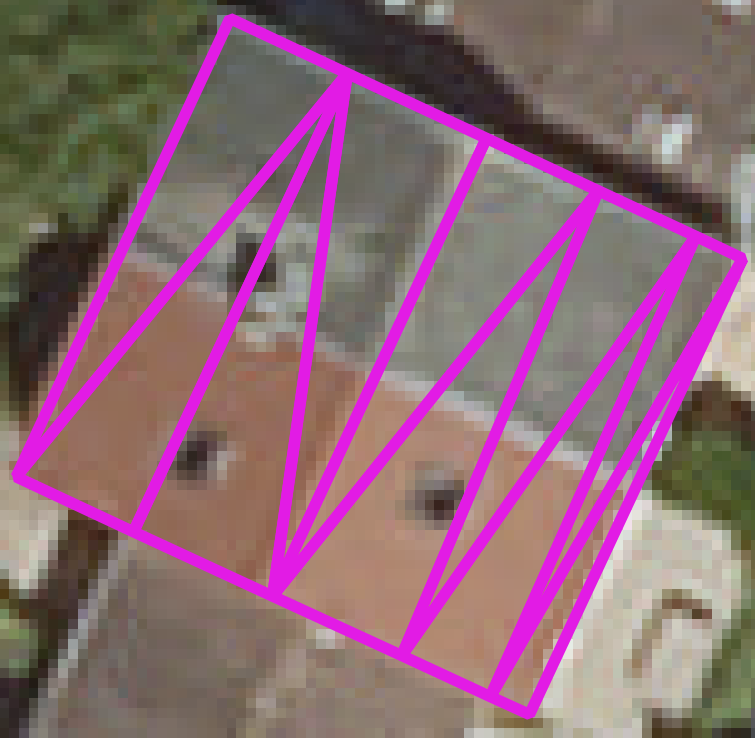
\includegraphics[height=.11\textheight]{images/Building_Errors/under_segmentation}}
                        \ffigbox[\FBwidth]{\caption{\textit{BOS}}\label{fig::over_bul}}{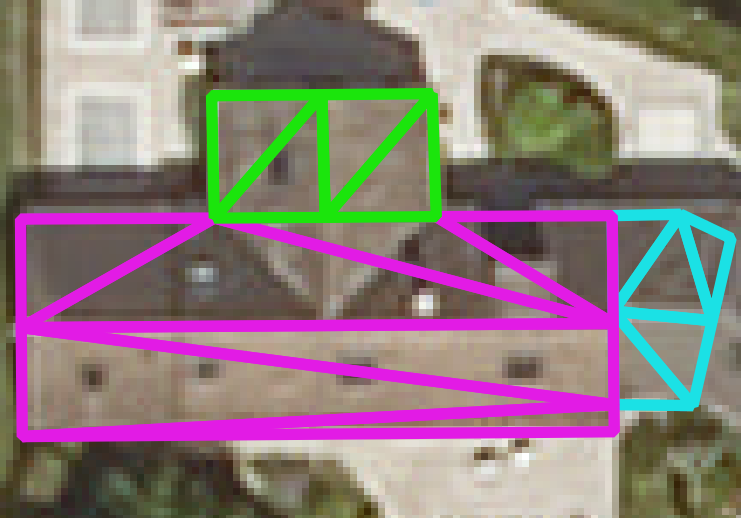
\includegraphics[height=.11\textheight]{images/Building_Errors/over_segmentation}}
                        \ffigbox[\FBwidth]{\caption{\textit{BInF}}\label{fig::footprint}}{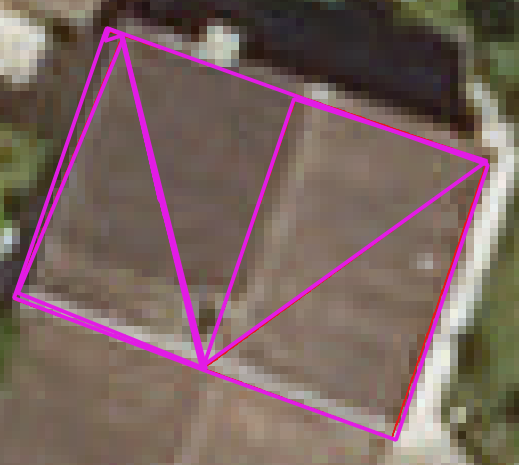
\includegraphics[height=.11\textheight]{images/Building_Errors/footprint}}
                        \ffigbox[\FBwidth]{\caption{\textit{BImH}}\label{fig::height}}{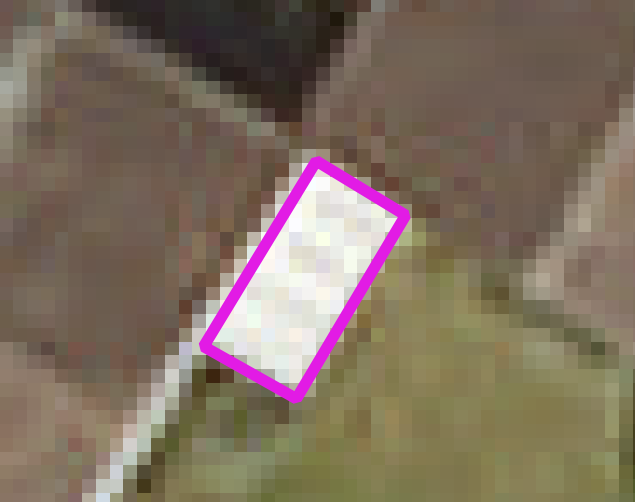
\includegraphics[height=.11\textheight]{images/Building_Errors/altimetric}}
                    \end{subfloatrow}
                }
                {
                    \captionsetup{labelfont={tiny, bf},textfont=scriptsize,justification=raggedright, labelsep=period}
                    \renewcommand{\thesubfigure}{\roman{SubFigCounter}}
					\vspace{-.3cm}
                    \captionof{subfigure}{Building errors family samples.}\label{fig::bul_err}
                    \refstepcounter{SubFigCounter}
                    \addtocounter{figure}{-1}
                }
                \ffigbox[\FBwidth]
                {
                    \begin{subfloatrow}[4]
                        \ffigbox[\FBwidth]{\caption{\textit{FUS}}\label{fig::under_fac}}{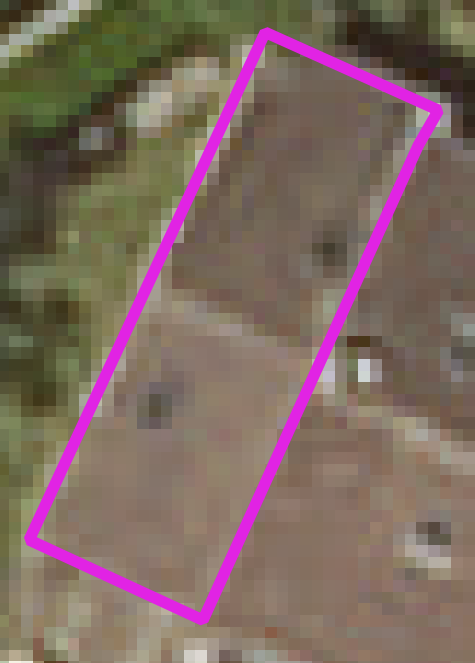
\includegraphics[height=.11\textheight]{images/Facet_Errors/under_segmentation}}
                        \ffigbox[\FBwidth]{\caption{\textit{FOS}}\label{fig::over_fac}}{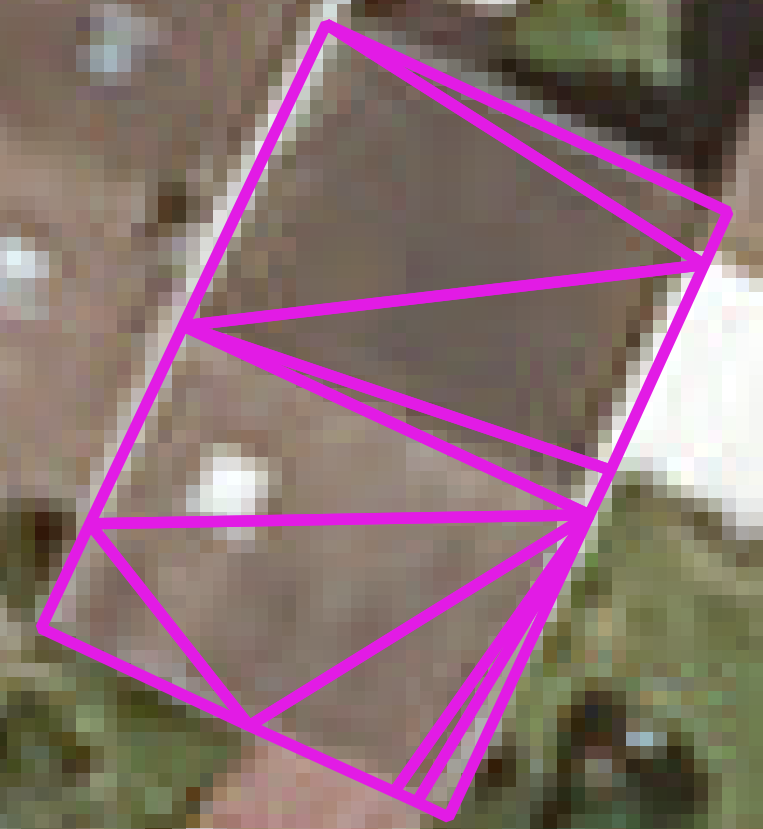
\includegraphics[height=.11\textheight]{images/Facet_Errors/over_segmentation}}
                        \ffigbox[\FBwidth]{\caption{\textit{FIS}}\label{fig::mis}}{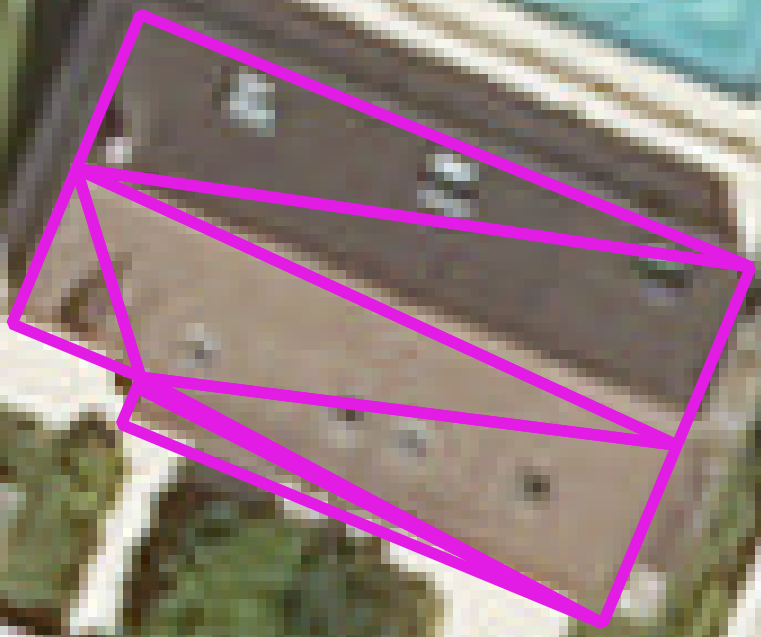
\includegraphics[height=.11\textheight]{images/Facet_Errors/mis_segmentation}}
                        \ffigbox[\FBwidth]{\caption{\textit{FImS}}\label{fig::slope}}{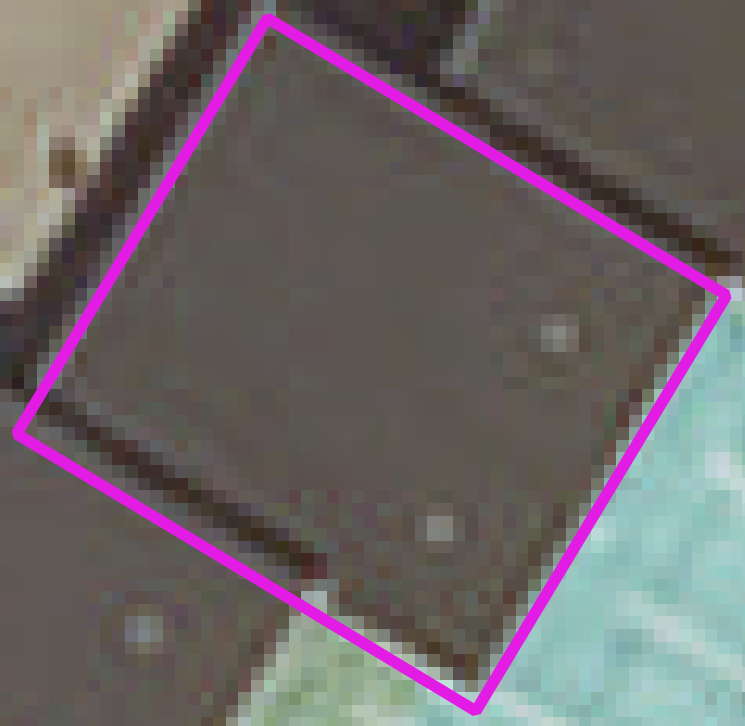
\includegraphics[height=.11\textheight]{images/Facet_Errors/slope}}
                    \end{subfloatrow}
                }
                {
                	\captionsetup{labelfont={bf},justification=raggedright, labelsep=period}
                    \renewcommand{\thesubfigure}{\roman{SubFigCounter}}
					\vspace{-.3cm}
                    \captionof{subfigure}{Facet errors family samples.}\label{fig::fac_err}
                    \refstepcounter{SubFigCounter}
                    \addtocounter{figure}{-1}
                }
            }
            {
                \caption{\label{fig::samples}Illustration of various errors of our taxonomy. One can see that geometric, spectral and height information are required for an accurate detection of all kinds of errors.}
            }
        \end{center}
    \end{figure*}

\subsection{Feature baseline}

	We propose a simple baseline of features as we try to prove if this pipeline is promising for further investigation. We rely on three modalities. The first is the input model itself. We extract statistics (maximum, minimum, mean, median and standard deviation) over attributes that describe the geometry of the building facets: number of nodes, area, angle between normals, distance between centroids and circumference. We can further add to these geometric features altimetric ones. These are represented by the histogram of the discrepancy between the 3D model height-map and the corresponding \acrshort{acr::dsm} at the same spatial resolution. Looking for robustness, this resolution are chosen to be lower than building dimensions but higher than the modeling inherent planimetric uncertainty. Last comes optical features, these are computed by back-projecting the input model on corresponding orthoimages. For each facet edge we compute a correlation histogram to image edges using the cosine similarity between local gradients and the edge normal. This histogram is summed over all facet edges and then over all projected facets. The more the histogram is concentrated near the value $1$ the more facet edges correspond to real image ones.

\subsection{Classification process}

	The extracted error labels extracted from the taxonomy are organized into different classification problems as showed in Table~\ref{tab::problems}.
\begin{table*}
	\begin{center}
		\begin{tabular}{c c c x{8cm}}
			\toprule
            \textbf{\textit{finesse}} & \textbf{\acrshort{acr::elod}} & \textbf{exclusivity} & \textbf{Classification output}\\
            \midrule
            \scriptsize
            $1$ & -- & -- & Binary(Valid, Erroneous)\\
            $2$ & \acrshort{acr::lod}-$1$ & -- & Binary(Valid, Building error)\\
            $2$ & \acrshort{acr::lod}-$2$ & on & MultiClass(Valid, Building error, Facet error)\\
            $2$ & \acrshort{acr::lod}-$2$ & off & MultiLabel(Valid, Building error, Facet error)\\
            $3$ & \acrshort{acr::lod}-$1$ & on & MultiLabel(children(Binary(Valid, Building error)))\\
            $3$ & \acrshort{acr::lod}-$2$ & on & MultiLabel(children(MultiClass(Valid, Building error, Facet error)))\\
            $3$ & \acrshort{acr::lod}-$1$ & off & MultiLabel(children(Building error))\\
            $3$ & \acrshort{acr::lod}-$2$ & off & MultiLabel(children(Building error)$\cup$ children(Facet error))\\
            \bottomrule
		\end{tabular}
        \caption{\label{tab::problems} The summary of all possible classification problem types. children($error$) lists the children of $error$ from the taxonomy tree (Figure~\ref{fig::taxonomy}).}
	\end{center}
\end{table*}

The different modalities provide each $20$ dimensional vectors. To account for the desired modularity and flexibility, a random forest classifier~\cite{breiman2001random} is chosen using 1,000 trees and a maximal depth of 4. The depth is kept shallow in order to avoid overfitting while the big number of estimators deals with the large feature space variability. The Multi-label setting is managed using a One vs All strategy on top of our classifier.

\section{Experiments}
\label{sec:expe}

We evaluate our approach using a 3D city model over the city of \textcolor{red}{Elancourt (France). The studied scene spans an area of \SI{15}{\km\squared}. It exhibits a high diversity of building types and errors: residential districts with mostly bi-level buildings, industrial areas with flat roof buildings, a stadium, a petrol station and administrative edifices such as schools.} These were modeled, using the algorithm described in~\cite{Durupt2006}, out of existing building footprints and an aerial multi-view \acrshort{acr::dsm} with a \SI{0.06}{\m} spatial resolution. \textcolor{red}{1,501} buildings are considered in these experiments. They were annotated according to the atomic errors list provided by our taxonomy.

Based on the devised pipeline, four feature configurations were tested: ``geometric features'' only, ``geometric and height features'', ``geometric and image features'' as well as ``geometric, height and image features''. A \SI{0.06}{\m}/\SI{0.10}{\m} spatial resolution \acrshort{acr::dsm} and integral orthorectified image are used to derive altimetric and optical features. Labels are extracted from a non \textbf{exclusive} and \textbf{\acrshort{acr::elod}} $=$ \acrshort{acr::lod}-$2$ taxonomy. We report here only the \textit{finesse} level of $3$. We perform a $10$-fold cross validation.
\begin{table*}
	\scriptsize
	\begin{center}
        \begin{tabular}{|x{1.4cm} | x{1.2cm} x{1.2cm} | x{1.2cm} x{1.2cm} | x{1.2cm} x{1.2cm} | x{1.2cm} x{1.2cm}|}
			\hline
            &\multicolumn{2}{x{2.4cm}|}{\textbf{Geometry}} & \multicolumn{2}{x{2.4cm}|}{\textbf{Geom. $\cup$ Height}} & \multicolumn{2}{x{2.4cm}|}{\textbf{Geom. $\cup$ Image}} & \multicolumn{2}{|x{2.4cm}|}{\textbf{All}}\\
            \cline{2-9}
            &\textbf{Recall} & \textbf{Prec.} & \textbf{Recall} & \textbf{Prec.} & \textbf{Recall} & \textbf{Prec.} & \textbf{Recall} & \textbf{Prec.}\\
            \hline
            \textit{BOS} & \textbf{94.34} & $77.09$ &$93.36$ & \textbf{77.66} &$92.38$ & $77.04$ &$92.19$ & $76.69$ \\
            \hline
            \textit{BUS} & $34.38$ & $76.43$ &$31.52$ & \textbf{78.57} & \textbf{42.98} & $76.53$ &$41.55$ & $77.96$ \\
            \hline
            \textit{BIFoB} & \textbf{22.34} & \textbf{68.85} & $22.34$ & $67.74$ &$18.09$ & $64.15$ &$18.62$ & $64.81$ \\
            \hline
            \textit{BIFoT} & \textbf{22.34} & \textbf{68.85} & $22.34$ & $67.74$ &$18.09$ & $64.15$ &$18.62$ & $64.81$ \\
            \hline
            \hline
            \textit{FOS} & $98.77$ & \textbf{98.77} & \textbf{98.87} & $98.67$ &$98.67$ & $98.47$ &$98.67$ & $98.37$ \\
            \hline
            \textit{FUS} & \textbf{0.70} & \textbf{50.00} &$0.70$ & $33.34$ & \textbf{0.70} & \textbf{50.00} & \textbf{0.70} & \textbf{50.00} \\
            \hline
            \textit{FIFoB} & \textbf{1.36} & \textbf{66.67} &$1.36$ & $50.00$ &$1.36$ & $28.57$ &$1.36$ & $40.00$ \\
            \hline
            \textit{FIFoT} & \textbf{1.36} & \textbf{66.67} &$1.36$ & $50.00$ &$1.36$ & $28.57$ &$1.36$ & $40.00$ \\
            \hline
            \textit{FIG} & $0$ & --- & $0$ & --- & $0$ & --- &$0$ & --- \\
            \hline
		\end{tabular}
	\end{center}
    \vspace{-.5cm}
    \caption{\label{tab::f3_res}Results (\%) for the \textit{finesse} level $3$. All \textit{atomic} errors are considered over all possible configurations.}
\end{table*}

Discussion results.

Qualitative assessment is also performed in order to illustrate some failure cases (Figure~\ref{fig::results}, from left to right). In the first image, the similarity of the building outline to over segmented buildings cases induces an overdetection. In the second example, the building is wrongfully detected as being under segmented due to the presence of a balcony and a smaller annex building. In the third building, while correctly predicting \textit{BOS}, our algorithm fails to detect the under segmented roof. Finally, in the last depiction, except the well caught footprint error, defects are overlooked as there are few comparable samples in the dataset. To alleviate these issues, more robust features could be introduced taking into account higher order information. Dataset enrichment could be another option which provides more instances of underrepresented errors. In the end, we can also add the human in the loop through manual interactive evaluation which can adapt well to user-specific needs.

\begin{figure*}
	\begin{center}
    \tiny
		\begin{tabular}{| x{1.11cm} | x{.75cm} | x{.75cm} || x{1.11cm} | x{.75cm} | x{.75cm} || x{1.11cm} | x{.75cm} | x{.75cm} || x{1.11cm} | x{.75cm} | x{.75cm} |}
			\hline
			\multicolumn{3}{| c ||}{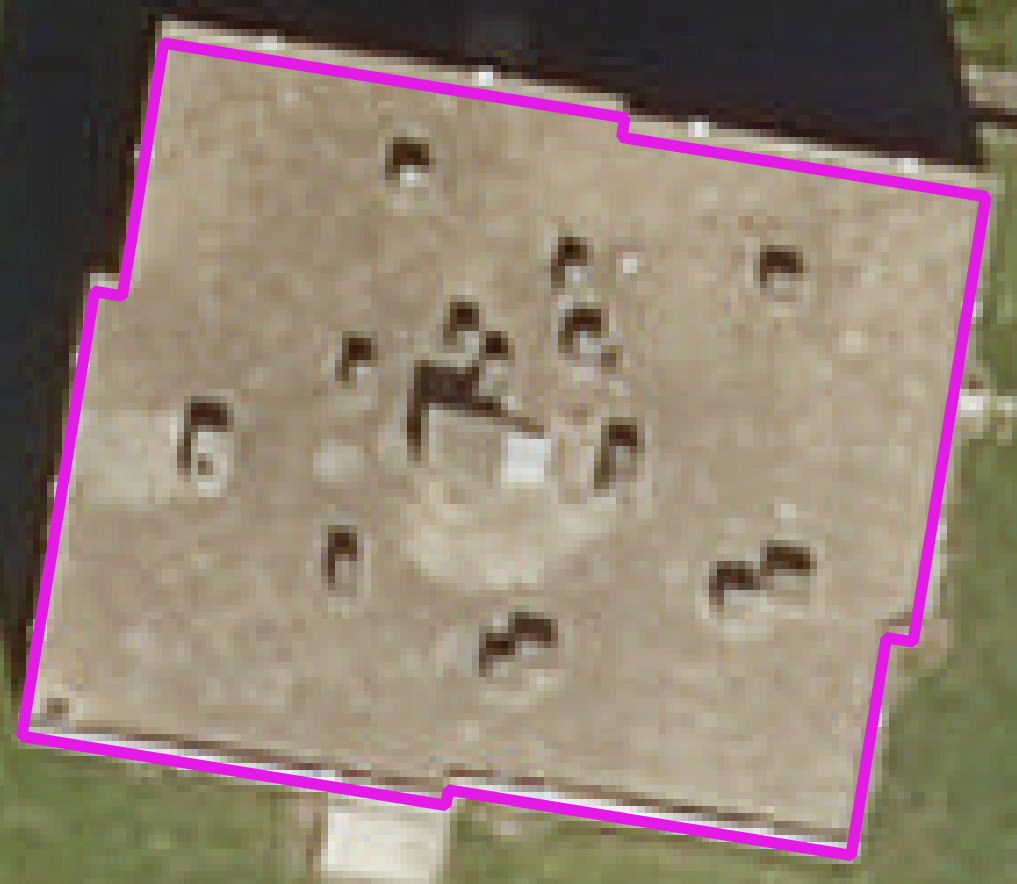
\includegraphics[height=.1\textheight,valign=m,margin=.1cm .1cm]{images/prediction_results/valid_as_bul_over}} & \multicolumn{3}{ c ||}{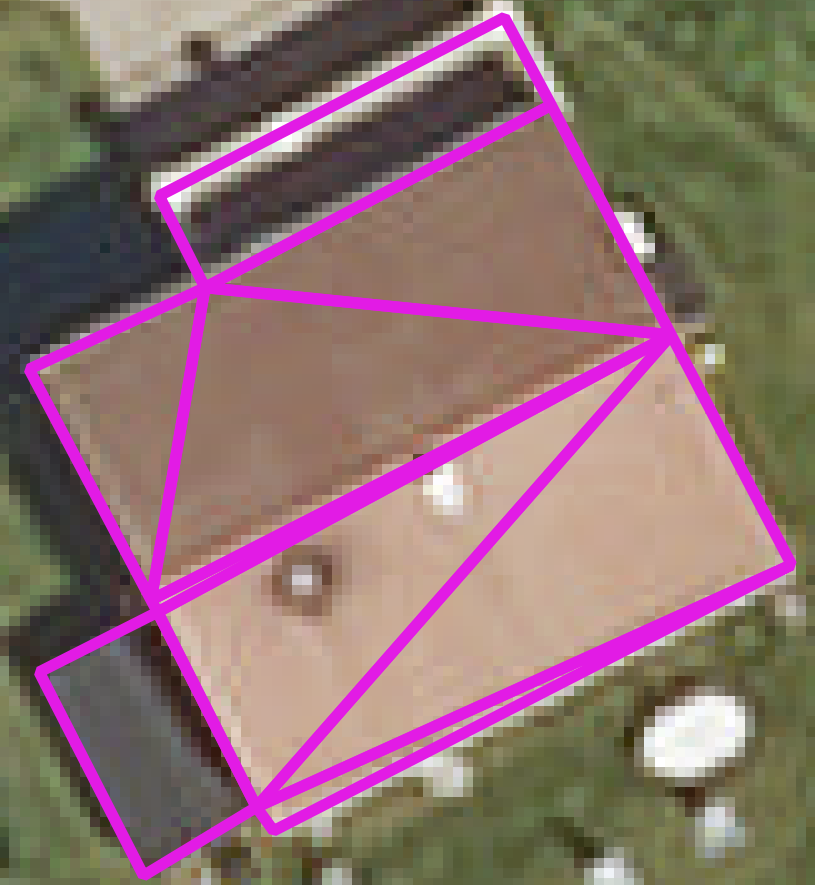
\includegraphics[height=.1\textheight,valign=m,margin=0cm .1cm]{images/prediction_results/no_imprec_no_fac_over}} & \multicolumn{3}{ c ||}{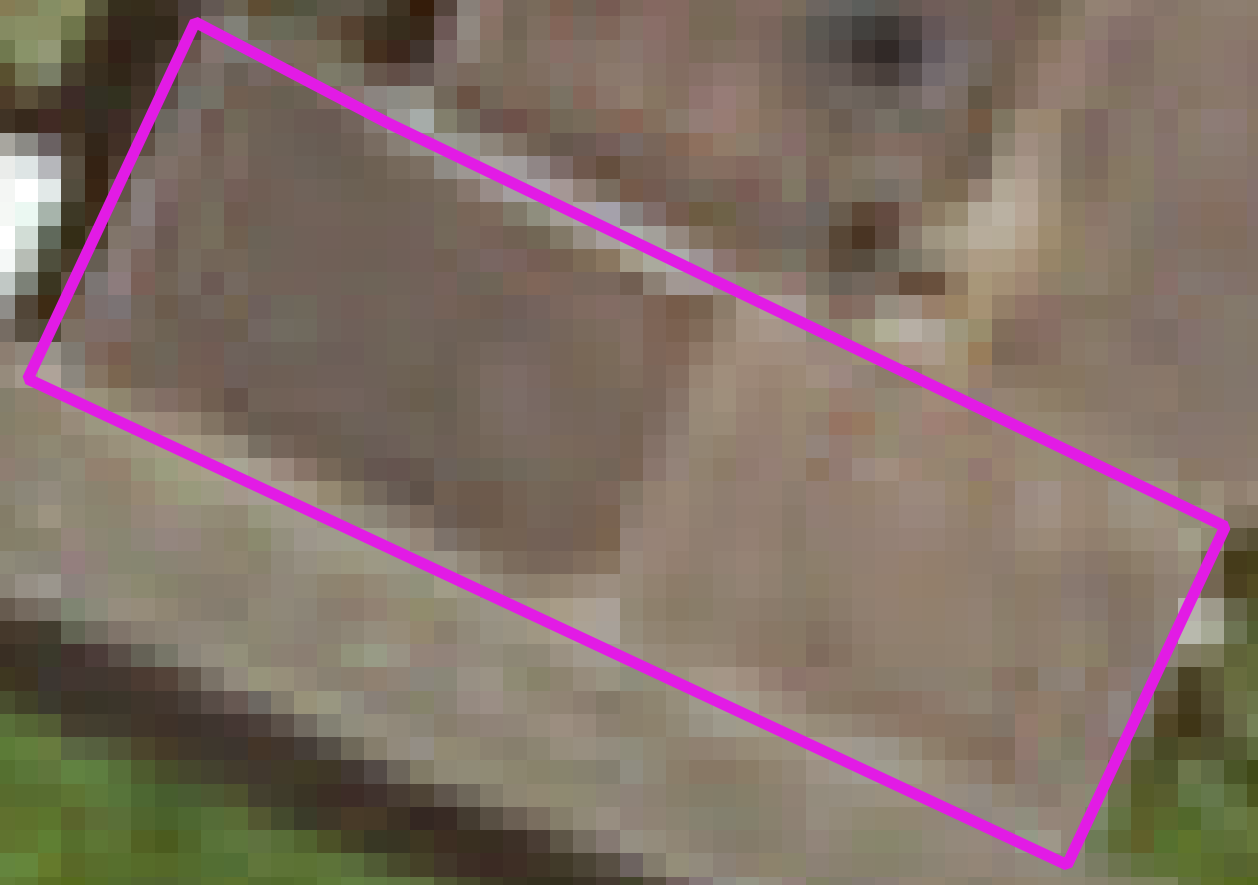
\includegraphics[height=.1\textheight,valign=m,margin=0cm .1cm]{images/prediction_results/no_under_seg}} & \multicolumn{3}{ c |}{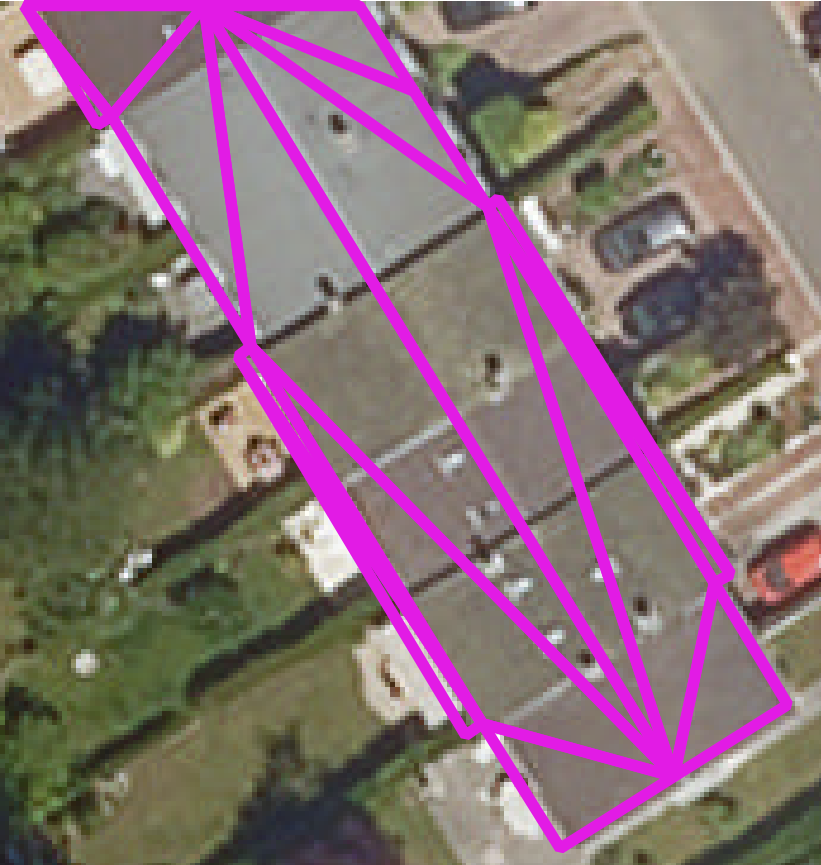
\includegraphics[height=.1\textheight,valign=m,margin=0cm .1cm]{images/prediction_results/no_bul_under_seg}} \\
			\hline
			\textbf{Errors} & \textbf{G.T.} & \textbf{Pred.} & \textbf{Errors} & \textbf{G.T.} & \textbf{Pred.} & \textbf{Errors} & \textbf{G.T.} & \textbf{Pred.} & \textbf{Errors} & \textbf{G.T.} & \textbf{Pred.}\\
            \hline
            \textit{BOS} & \xmark & \cmark & \textit{BUS} & \xmark & \cmark & \textit{BOS} & \cmark & \cmark & \textit{BOS} & \cmark & \xmark \\
            Valid & \cmark & \xmark & \textit{FImS} & \cmark & \xmark & \textit{FUS} & \cmark & \xmark &  \textit{FOS} & \cmark & \xmark \\
             &  &  & \textit{FOS} & \cmark & \xmark &  &  &  & \textit{BUS} & \cmark & \xmark \\
             &  &  &  &  &  &  &  &  &  \textit{BInF} & \cmark & \cmark \\
            \hline
		\end{tabular}
        \vspace{-.5cm}
        \caption{\label{fig::results} Predicted (Pred.) errors compared to ground truth (G.T.) labels are illustrated for some pathological cases. Knowing how each error is represented in the dataset helps interpreting mispredictions.}
	\end{center}
\end{figure*}

\section{Conclusion}
\label{sec::conclusion}

We proposed a framework to semantically evaluate automatically modeled buildings. For that purpose, errors are hierarchically organized into a flexible and parametrized taxonomy. It aims to handle the large diversity of urban enviroments and varying requirements.% stemming from end-users (geometric accuracy and level of details). Based on the desired \acrshort{acr::lod}, exclusivity and semantic level, an error collection is considered. 
Model quality was predicted using a supervised classifier. Each model provides intrinsic geometrical characteristics that are compiled in a feature vector. Other modalities can help describing building models, as attributes can also be extracted from model comparison to images or depth data. It helps detecting hard cases.

%This new framework was applied to the case of aerial urban reconstruction, where features are extracted from geospatial images and a \acrshort{acr::dsm}. A dataset containing $1,501$ aerial reconstructed building models with high diversity was used to test the devised evaluation method associated to multimodal baseline features.
Although being mitigated over under-represented errors, results are satisfactory in the well balanced cases. As a next step, more structurally aware features (based on graph comparison, for instance) could be proposed so as to be applied on a richer and more diverse dataset (potentially involving data augmentation) under a deep-based framework.

\bibliographystyle{IEEEtran}
\bibliography{IEEEabrv,references}
\end{document}
